\chapter{Trabalhos Relacionados}
\label{ch:relacionados}

Esta seção apresenta trabalhos relacionados a com o modelo proposto, bem como uma comparação entre os mesmos.

\section{PeLeP}

O projeto PeLeP, apresentado por \citetexto{pelep}, integra a utilização de perfis aperfeiçoados automaticamente com ambientes de educação ubíqua.

Barbosa et al compreendem \emph{educação ubíqua} como sendo processos educacionais que ocorrem em qualquer lugar, a qualquer tempo e com qualquer dispositivo, de forma contínua, contextualizada e integrada ao cotidiano do aprendiz. Desta forma, o conhecimento presente no dia-a-dia das mais diferentes formas e em diferentes locais podem ser relacionados com processos educacionais direcionados aos aprendizes \cite{barbosa05}.

O PeLeP, cujo modelo é ilustrado na Figura~\ref{fig:pelep1}, é dedicado ao gerenciamento de perfis de aprendizes em um ambiente ubíquo de ensino e aprendizagem. O modelo administra os perfis automaticamente, inferindo informações através do histórico do aprendiz. As alterações realizadas no perfil refletem o comportamento do aprendiz no ambiente ubíquo, levando em consideração o seu modelo de mobilidade e de contexto.

\begin{figure}
  \centering
  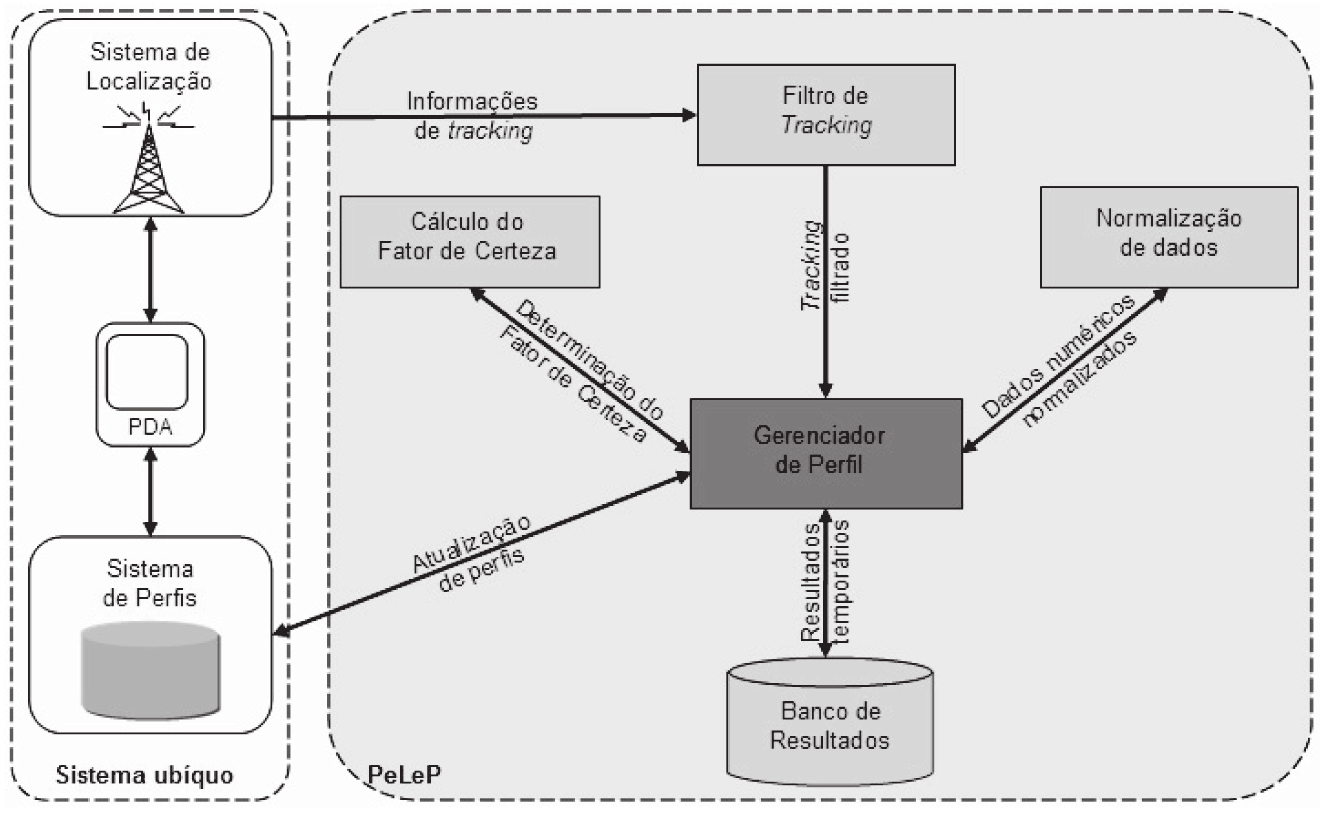
\includegraphics[width=0.8\textwidth]{imagens/pelep1.png}
  \caption{Arquitetura do PeLeP\cite{pelep}}
  \label{fig:pelep1}
\end{figure}

No PeLeP, o \emph{perfil do aprendiz} consiste em um perfil contendo campos pré-definidos, voltados para o ambiente de educação ubíqua. Os campos são distribuídos nas seguintes categorias: identificação, objetivos, agenda, segurança, relacionamentos, competências e preferências. 

É realizado um acompanhamento (\emph{tracking}) do histórico do aprendiz, onde são armazenados os contextos visitados pelo usuário, bem como os conteúdos, dispositivos e aplicativos utilizados em cada contexto. Os valores relativos das variáveis numéricas recebidas no \emph{tracking} são regularizados através de um processo de normalização de amplitude. Como diferentes valores podem ter diferentes impactos para a determinação da preferência de um usuário, calcula-se o Fator de Certeza ($FC$), de acordo com a equação~\ref{eq:pelep-fc}, onde $f_i$ é o valor normalizado para o fator, $p_i$ o seu percentual, e $n$ o número de fatores considerados.

\begin{equation}
  FC = \frac{\frac{\displaystyle\sum_{i=0}^n f_i p_i}{100}}{n}
  \label{eq:pelep-fc}
\end{equation}

O fator tempo também é levado em consideração, onde Fatores de Certeza mais antigos tem um impacto menor. Assim, por exemplo, se o usuário trocar o seu aplicativo preferido, à medida que o tempo for passando o impacto do aplicativo anterior será cada vez menor.

O processo de atualização do modelo do aprendiz é então realizado através de regras pré-definidas, que levam em conta as ocorrências e o seu fator de certeza. As regras suportam conclusões a partir de evidências antecedentes, e cada categoria de informação possui regras diferentes.

O PeLeP foi validado através da integração com o Local ({\em Location and Context-Aware Learning}), um sistema de educação ubíqua sensível a contexto \cite{barbosa08}.

%%%%%%%%%%%%%%%%%%%%%%%%%%%%%%%%%%%%%%%%%%%%%%%%%%%%%%%%%%%%%%%%%%%%%%%%%

\section{Chellouche et al}

O artigo de \citetexto{chellouche10} discute as dificuldades atuais no desenvolvimento de aplicativos para dispositivos móveis, uma vez que os mesmos possuem uma grande variedade de resolução, memória, poder computacional, entre outros. Além disso, a qualidade da conexão de um usuário pode variar significativamente, e isto também deve ser levado em consideração no desenvolvimento.

O conjunto de informações que caracteriza um usuário é chamada de \emph{perfil de usuário}. Com a intenção de compartilhar o contexto do usuário entre serviços e minimizar as mudanças no desenvolvimento de aplicações sensíveis a contexto, os autores propõem como solução um \emph{middleware} que gerencia o perfil de um usuário dinamicamente e supre às aplicações todas as informações que elas podem precisar durante o período de adaptação.

O perfil do usuário é constituído por seu contexto, onde a definição de contexto utilizada é aquela dada por \citetexto{dey2001}, na qual contexto refere-se a qualquer informação que pode ser utilizada para caracterizar a situação de uma entidade. Assim, o perfil de usuário é dividido em cinco componentes:

\begin{description}
  \item[Perfil geral:] refere-se às informações básicas, como nome, endereço, telefone, idade, sexo, entre outros;
  \item[Perfil do dispositivo:] contém informações a respeito dos dispositivos do usuário, tais como marca, capacidade, sistema operacional, entre outros;
  \item[Perfil de rede:] descreve as redes às quais o usuário pode se conectar, com suas características;
  \item[Perfil dos serviços:] registra as informações a respeito de serviços, como nome, versão, porta e conteúdo;
  \item[Perfil de contexto:] contém informações a respeito do ambiente do usuário, como hora, data e localização, aplicações em execução e banda disponível. É considerada a parte dinâmica do perfil, composta por dados voláteis.
\end{description}

O \emph{middleware} é apresentado segundo ilustrado na Figura~\ref{fig:chellouche1}. O \emph{middleware} é composto dos seguintes módulos:

\begin{figure}
  \centering
  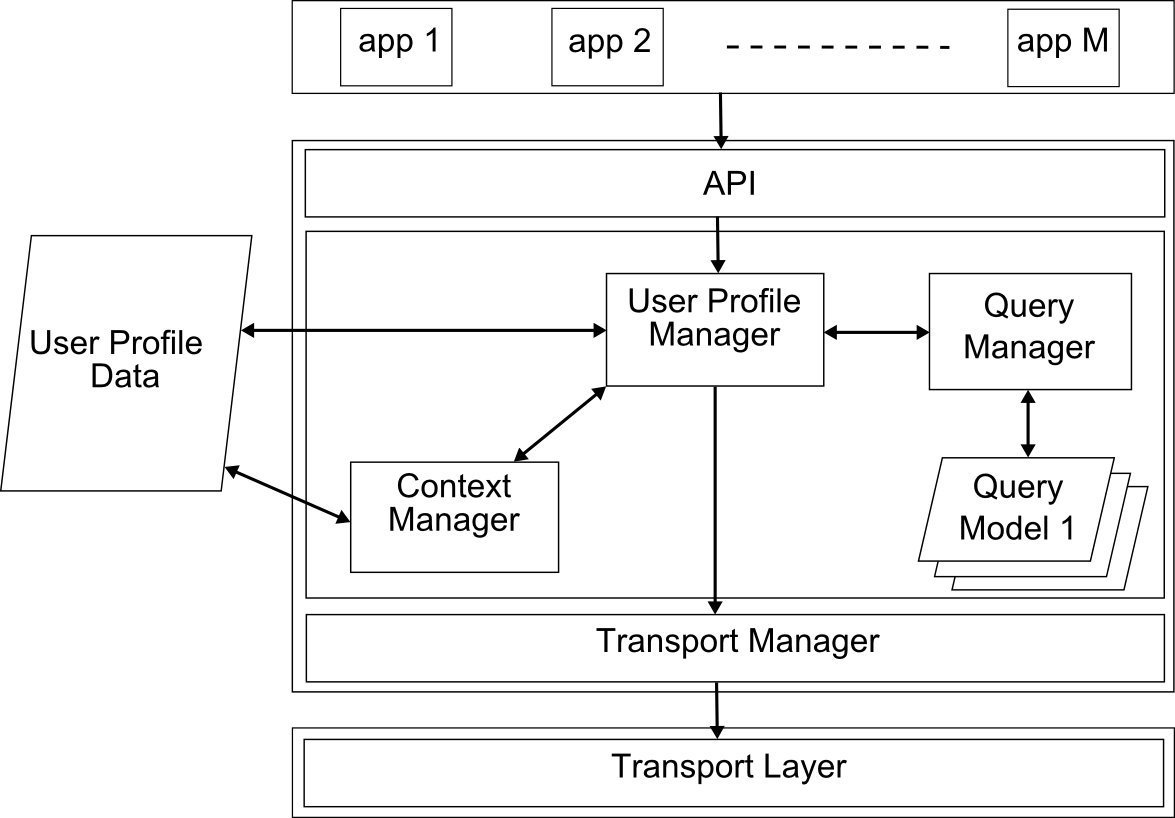
\includegraphics[width=0.8\textwidth]{imagens/chellouche1.png}
  \caption{Arquitetura do \emph{middleware} de \citetexto{chellouche10}}
  \label{fig:chellouche1}
\end{figure}

\begin{description}
  \item[Gerenciador de perfil de usuário:] módulo central da arquitetura, que interage com todos os outros módulos com o objetivo de construir o perfil correto;
  \item[Gerenciador de contexto:] monitora o ambiente, coletando informações com o objetivo de atualizar a parte dinâmica do perfil;
  \item[Gerenciador de consultas:] módulo responsável por validar e salvar um modelo de consulta para cada aplicação;
  \item[Gerenciador de trasporte:] faz a comunicação do perfil de usuário para a aplicação;
  \item[API]: constitui o ponto de interface entre as aplicações e o \emph{middleware}.
\end{description}

O perfil é construído de acordo com a Figura~\ref{fig:chellouche2}. A aplicação solicita os dados ao gerenciador de perfis, através da API, que por sua vez repassa a solicitação ao gerenciador de consultas. Ao mesmo tempo, o gerenciador de contextos é informado que a aplicação está em execução e passa a atualizar o gerenciador de perfis com as informações atualizadas. O perfil de usuário é criado e enviado ao gerenciador de transporte, que retorna o perfil solicitado à aplicação solicitante.

\begin{figure}
  \centering
  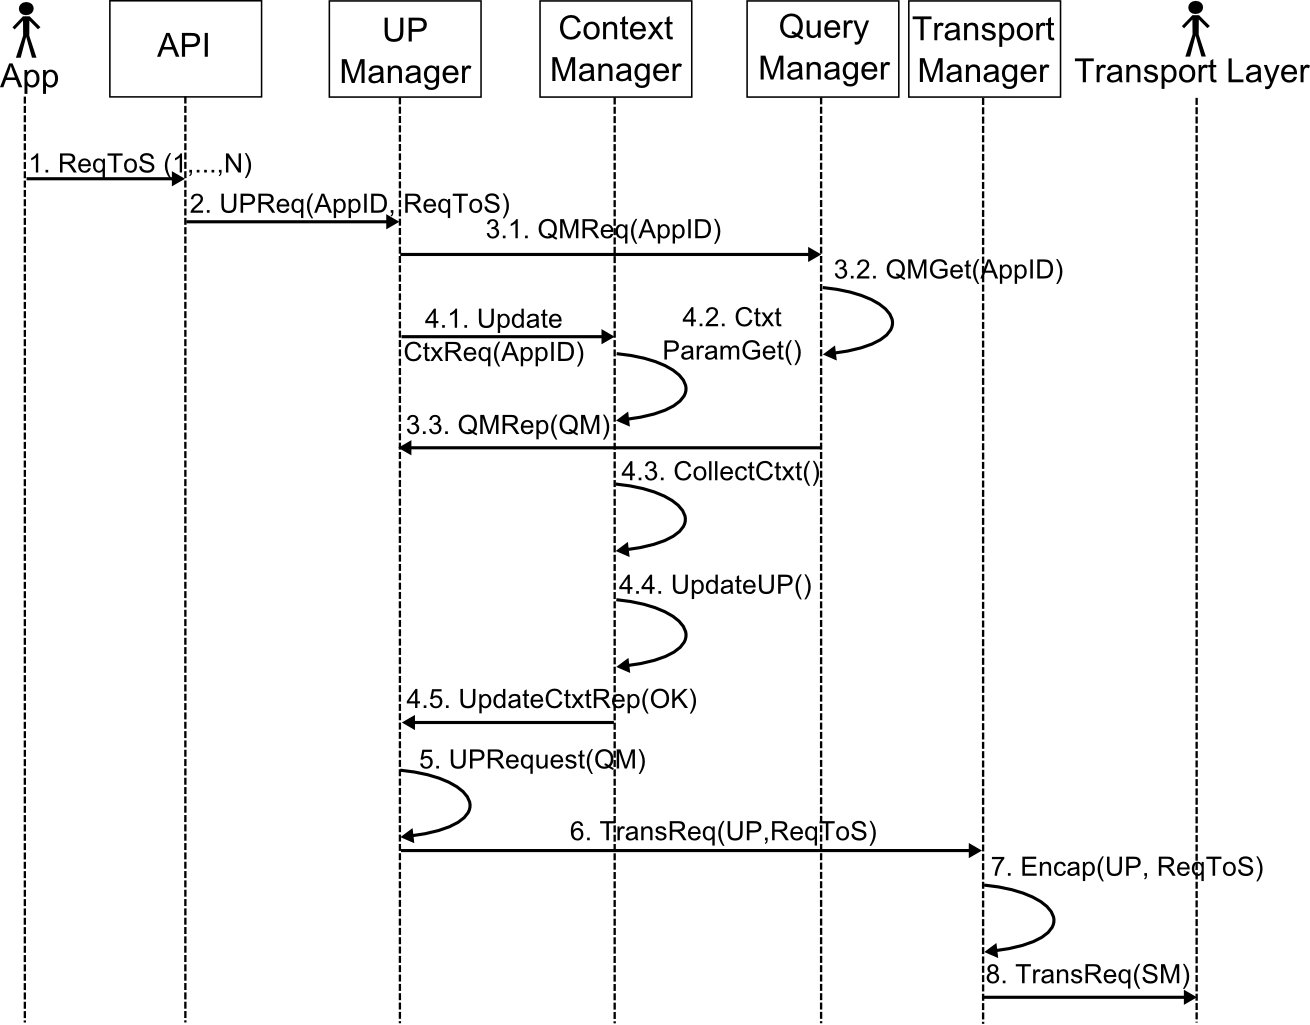
\includegraphics[width=0.8\textwidth]{imagens/chellouche2.png}
  \caption{Construção de perfil\cite{chellouche10}}
  \label{fig:chellouche2}
\end{figure}

%%%%%%%%%%%%%%%%%%%%%%%%%%%%%%%%%%%%%%%%%%%%%%%%%%%%%%%%%%%%%%%%%%%%%%%%%%

\section{UUCM}

O artigo apresentado por \citetexto{niederee04} busca responder três indagações, que são apresentadas como sendo os três desafios básicos da personalização:

\begin{itemize}
  \item Como modelar o usuário e sua situação de modo extensível e unificado, de forma que este modelo possa ser interpretado e usado para personalização por diferentes sistemas?
  \item Como coletar dados para preencher e atualizar perfis de usuário a partir das interações do usuário com diferentes sistemas baseados em um modelo de contexto de usuário unificado?
  \item Como habilitar conceitualmente e tecnicamente diferentes sistemas a fazer uso dos perfis de usuário coletados para aperfeiçoamento do suporte ao usuário?
\end{itemize}

Os autores apresentam como resposta a estas indagações um modelo denominado UUCM, que tem como objetivo modelar características do usuário e de seu contexto. O conceito de contexto utilizado é aquele apresentado por \citetexto{benerecetti00}, na qual o contexto pode ser pensado como as informações extras, geralmente implícitas (como associações, fatos, suposições), que podem ser utilizadas para compreender plenamente uma interação, comunicação ou representação de conhecimento.

A abordagem para a modelagem unificada de contextos de usuário é proposta em dois níveis. No nível \emph{abstrato}, são definidos os blocos básicos de construção: contexto de usuário, facetas do modelo de usuário, propriedades principais e dimensões do modelo de usuário. O termo faceta representa as diferentes características do usuário.  Este nível define um metamodelo para as dimensões e facetas concretas utilizadas na descrição do modelo de contexto de usuário. Para que a abordagem de personalização multi-sistema seja válida, é necessário que este metamodelo de contexto de usuário seja publicado como uma ontologia compartilhada, e que todos os participantes utilizem este modelo.

No nível \emph{concreto}, um conjunto de dimensões e facetas são definidos. As facetas e dimensões são descritas como parte de uma ontologia adicional que é compartilhada pelos componentes envolvidos na personalização multi-sistemas.

\begin{figure}
  \centering
  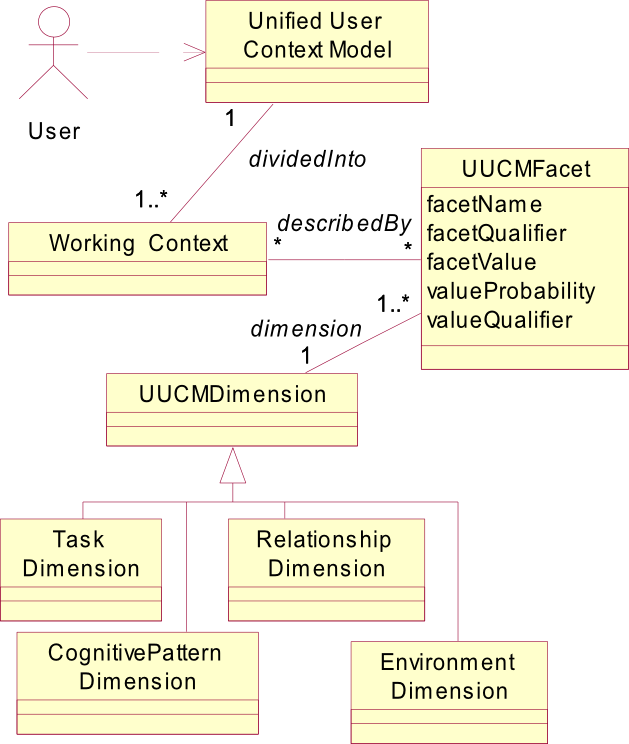
\includegraphics[width=0.5\textwidth]{imagens/niederee1.png}
  \caption{Modelo do UUCM \cite{niederee04}}
  \label{fig:niederee1}
\end{figure}

O modelo do UUCM é apresentado na Figura~\ref{fig:niederee1}. Segundo o modelo, um perfil de usuário (\emph{Unified User Context Model}) é dividido em um conjunto de contextos de trabalho (\emph{Working Contexts}), onde cada contexto é descrito por um conjunto de facetas (\emph{UUCM facet}). Cada faceta é vinculada a uma dimensão (\emph{UUCMDimension}).

O UUCM apenas define o método através do qual o perfil de contexto de usuário é descrito e estruturado para personalização multi-sistema. Para a descrição de perfis de contexto concretos, o UUCM utiliza ontologias (ou vocabulários) para as dimensões, facetas e valores de faceta.

As seguintes dimensões são utilizadas:

\begin{description}
  \item[Cognitiva] (\emph{CognitivePattern}): descreve as dimensões cognitivas do usuário, tais como \emph{áreas de interesse}, \emph{competências} e \emph{preferências};
  \item[Tarefa] (\emph{Task}): descreve os objetivos do usuário quando ele interage com sistemas. Utiliza dados tais como \emph{tarefa atual}, \emph{papel do usuário na tarefa} e \emph{histórico da tarefa};
  \item[Relacionamentos] (\emph{Relationship}): armazena as entidades com as quais o usuário tem alguma relação;
  \item[Ambiente] (\emph{Environment}): parâmetros que são tipicamente utilizados para abordagens sensíveis a contexto, tais como \emph{tempo}, \emph{localização}, \emph{dispositivo} e \emph{linguagem}.
\end{description}

O perfil de usuário do UUCM é codificado como um \emph{RDF Schema}\cite{rdf}, ampliado com expressões \emph{OWL}.

O modelo inclui ainda o conceito de \emph{passaporte de contexto}. O passaporte de contexto é uma representação compacta do modelo de contexto atual do usuário para a personalização multi-sistemas. Ele contém informações ontologicamente arranjadas a respeito dos padrões cognitivos (habilidades, interesses, etc), o ambiente (data, local, dispositivo usado) e sua rede pessoal de pessoas e relacionamentos envolvidos.

Para utilizar o passaporte de contexto em um ambiente de personalização multi-sistemas, o usuário ``apresenta'' o passaporte ao sistema que o usuário deseja utilizar. Como o passaporte está vinculado a uma ontologia compartilhada, é possível que o sistema consiga interpretar parcialmente o passaporte através de uma arquitetura mediadora. Como resultado, dois fluxos são possíveis: (i) do passaporte para o sistema, auxiliando o sistema a compreender o contexto do usuário, e (ii) do sistema para o passaporte, realizando alterações nas informações de contexto do usuário.

%%%%%%%%%%%%%%%%%%%%%%%%%%%%%%%%%%%%%%%%%%%%%%%%%%%%%%%%%%%%%%%%%%%%%%%%%%

\section{Avaliação dos Ambientes Pesquisados}

O PeLeP\cite{pelep} é um modelo que suporta o aperfeiçoamento automático do perfil do aprendiz em ambientes de educação ubíqua. Ele usa o histórico dos aprendizes nos contextos de um ambiente ubíquo para atualização dos perfis. O perfil do aprendiz no modelo é refinado e enriquecido através de inferências. As inferências são baseadas na mobilidade do aprendiz e no monitoramento das tarefas que ele executa nos contextos de um ambiente de educação ubíqua.

O modelo apresentado por \citetexto{chellouche10} apresenta um \emph{middleware} voltado para aplicações móveis que pode ser usado por diferentes aplicativos como um servidor central de perfis. Este modelo propõe como solução um \emph{middleware} que gerencia o perfil de um usuário dinamicamente e supre às aplicações todas as informações que elas podem precisar durante o período de adaptação.

O UUCM\cite{niederee04} é um modelo que pode ser utilizado para modelar as características de um usuário e seu contexto em ambientes de personalização de múltiplos sistemas. A proposta diz respeito a uma ontologia básica, baseada em contexto, a qual os sistemas podem estender, desde que os sistemas que usem este modelo concordem em uma ontologia básica.

Embora os modelos apresentados atualizem parte do perfil como forma de oferecer suporte a sensibilidade a contexto, nenhum deles permite que os aplicativos criem novos campos nem definam as regras para atualização dos campos existentes.

A Tabela~\ref{tab:comparacao} exibe um comparativo dos trabalhos apresentados, onde os seguintes fatores são levados em consideração:

% \todo[inline]{Descrever porque estes aspectos estão sendo avaliados.} % TODO

\begin{description}
  \item[Interoperabilidade:] considera se o modelo apresenta interoperabilidade -- caso positivo, se a mesma é sintática ou semântica;
  \item[Perfis dinâmicos:] identifica se o modelo de perfil permite que os perfis sejam atualizados de acordo com eventos externos, sem a interferência do usuário;
  \item[Armazenamento:] define onde ficam armazenados os perfis do usuário;
  \item[Sensível a contexto:] considera se o contexto do usuário é levado em consideração na formação do perfil;
  \item[Utiliza trilhas:] define se as trilhas do usuário são levadas em consideração na construção do perfil;
  \item[Domínio:] identifica se o perfil é voltado para um domínio específico, ou se o mesmo permite que vários domínios possam ser utilizados.
\end{description}

\begin{table*}\centering\footnotesize
  \begin{tabular*}{1\textwidth}{@{}lllllll@{}}
    \toprule
                                         & Interope-  & Perfis    & Armaze-  & Sensibilidade & Utiliza & \\
    Trabalho                             & rabilidade & dinâmicos & namento  & a contexto    & trilhas & Domínio \\
    \midrule
    PeLeP                                & Não        & Sim       & Servidor & Sim           & Parcial & Educação \\
    Chellouche et al                     & Sintática  & Sim       & Servidor & Sim           & Não     & Serviços multimídia \\
    UUCM                                 & Sintática  & Sim       & Cliente  & Sim           & Não     & Genérico \\
    \bottomrule
  \end{tabular*}
  \caption{Comparação entre os trabalhos apresentados}
  \label{tab:comparacao}
\end{table*}

